% !TeX root = ../thesis.tex

\chapter{Experimental Results}
\label{sec:evaluation}

Chapter \ref{sec:data_representation} presents various representations conceived within the scope of presented work to encode pixel-level relationships of instances. Chapter \ref{sec:experimentatl_setup} provides a brief overview of network architecture employed to learn these representations in combination with semantic segmentation and corresponding experimental setup. It further outlines the hyper-parameter specifications used for experiments carried out for evaluation purposes.  It is desired to evaluate the offset representations as well as distribution sizes and their affect on overall panoptic segmentation task. For a fair comparison and meaningful evaluation of results, manipulation of hyper-parameters across experiments is kept to a minimum. 

In this chapter results of experiments has been presented for evaluation purposes. Following section investigates various gaussian distribution sizes that were used to encode center-points and their affect on the task. A comparison between distribution sizes and performance on overall panoptic segmentation has been provided. Subsequently, the next section documents qualitative and quantitative analysis of different offset representations. Thereafter, an analysis on effects of different parameters used in post-processing step is provided. Based on lessons learned from experimentation with post-processing parameters and given the best post-processing and hyper-parameter settings, both offset representations and center points are evaluated against overall panoptic segmentation task. To the very end, a comparison between different feature extractor backbones and inference times has been provided.  


\bigskip



\section{Keypoints Evaluation}


\bigskip


In the presented work, instance segmentation which is a sub-task of panoptic segmentation relies heavily on center point predictions. Each instance mask generated by the presented bottom-up approach relies on a  center point pooled during non-maxima suppression as described in section \ref{subsec:center_rendering}. Therefore, learning on a reasonable center-point representation is critical for satisfactory performance of the model. As described in chapter \ref{sec:data_representation}, center points are encoded with a probability distribution around center points. To this end, comparative study has been carried out to investigate the right choice of distribution size. For a comparison purpose multiple datasets have been generated that encoded center points with guassian distribution of standard deviation 2, 4, 8 and 16. A comparison of these different variants with respect to overall panoptic task has been shown. Table \ref{tab:distribution_comparison} provides a comparison of models that were trained on different distribution sizes and their corresponding performance metric. Performance metric in this case is chosen to be \gls{pc}. The results document class-wise parsing covering against the above mentioned distribution sizes.  

An important mention here is the fact that each of the compared models uses same encoding type i.e center-to-end encoding, see section \ref{subsec:c2e}, hyper-parameters and post-processing parameters to generate panoptic segmentation, see chapter \ref{sec:experimentatl_setup} for details about experimental setup and parameter specifications.
\begin{table}[!htp]
  \resizebox{1 \textwidth}{!}{
  \begin{tabular}{@{}rcccccccccccccccccccc@{}}

  & \multicolumn{1}{P{90}{1.6cm}}{Road} &
    \multicolumn{1}{P{90}{1.6cm}}{Sidewalk} &
    \multicolumn{1}{P{90}{1.6cm}@{}}{Building} &
    \multicolumn{1}{P{90}{1.6cm}}{Wall} &
    \multicolumn{1}{P{90}{1.6cm}}{Fence} &
    \multicolumn{1}{P{90}{1.6cm}@{}}{Pole} &
    \multicolumn{1}{P{90}{1.6cm}}{Traffic Light} &
    \multicolumn{1}{P{90}{1.6cm}}{Traffic Sign} &
    \multicolumn{1}{P{90}{1.6cm}@{}}{Vegetation} &
    \multicolumn{1}{P{90}{1.6cm}}{Terrain} &
    \multicolumn{1}{P{90}{1.6cm}}{Sky} &
    \multicolumn{1}{P{90}{1.6cm}@{}}{Person} &
    \multicolumn{1}{P{90}{1.6cm}}{Rider} &
    \multicolumn{1}{P{90}{1.6cm}}{Car} &
    \multicolumn{1}{P{90}{1.6cm}@{}}{Truck}&
    \multicolumn{1}{P{90}{1.6cm}}{Bus} &
    \multicolumn{1}{P{90}{1.6cm}@{}}{Train} &
    \multicolumn{1}{P{90}{1.6cm}}{Motorcycle} &
    \multicolumn{1}{P{90}{1.6cm}}{Bicycle} &
    \multicolumn{1}{P{90}{1.6cm}@{}}{ \textbf{Mean}}\\
      \midrule
        $\mathbf{\sigma = 2}$ &97.6&82.4&90.0&50.0&55.9&42.8&56.5&63.9&90.3&63.23&93.0&39.0&41.5&55.8&69.7&46.9&29.1&39.6&36.1&60.2 \\
        $\mathbf{\sigma = 4}$ &97.8&83.7&90.8&52.8&54.6&50.7&59.3&68.2&91.1&63.3&93.9&42.7&43.4&61.1&66.1&61.2&64.1&42.0&36.7&64.4  \\
        $\mathbf{\sigma = 8}$ &97.7 &83.6&90.3&52.9&53.7&48.7&54.3&66.2&90.7&61.3&93.1&45.2&41.2&64.3&73.3&65.0&66.7&40.9&38.2&\textbf{64.6} \\
        $\mathbf{\sigma = 16}$ &96.2&76.1&88.1&44.7&49.3&35.5&50.4&58.2&89.1&60.18&91.6&43.8&37.5&59.9&63.5&52.6&30.1&37.8&36.0&57.9 \\

  \bottomrule
  \end{tabular}
  }
  \caption[Comparison of Distribution Sizes for Center Points]{
  Comparison of models trained on different distribution sizes and corresponding class-wise parsing covering results showing that model trained on distribution with a standard deviation $\sigma = 8$ pixels has the best result.}
  \label{tab:distribution_comparison}
\end{table}

\paragraph{Discussion}

The overall comparison suggests that model that was trained on center points with guassians of standard deviation $\sigma = 8$-pixels resulted in the best performance for cityscapes dataset \cite{Cordts2015}. Center point predictions were scaled between $0$ and $1$ and thresholded at $0.39$ for the purpose of non-maxima suppression (NMS). Pooling window to extract exact center locations was set to be $64\times64$ pixels. 

\begin{figure}[!ht]
\centering
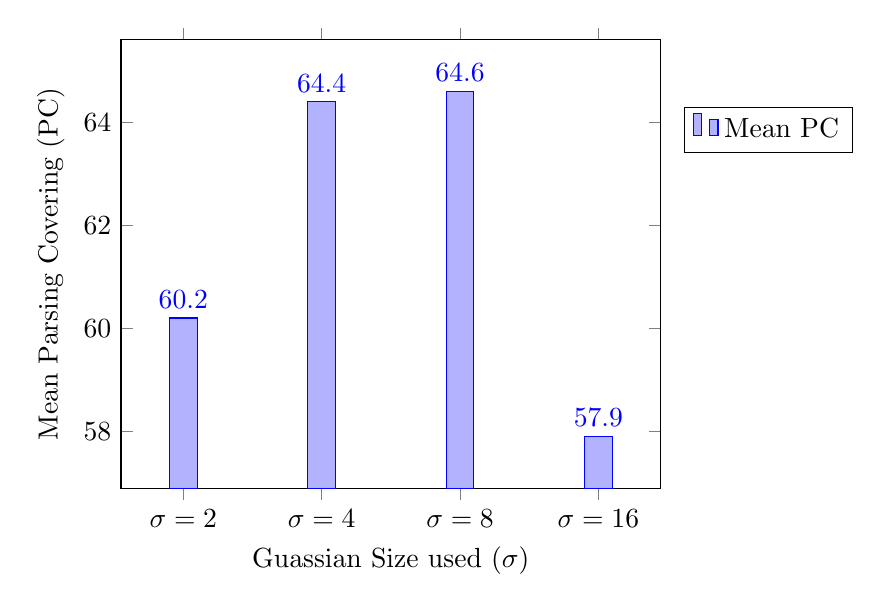
\begin{tikzpicture}  
\begin{axis}  
[      ybar,  
    enlargelimits=0.15,
    legend style={at={(1.2, 0.85)},
    anchor=north,legend columns=-1},
    ylabel={Mean Parsing Covering (PC)}, % the ylabel must precede a # symbol.  
    xlabel={Guassian Size used  $(\sigma)$},  
    symbolic x coords={$\sigma = 2$, $\sigma = 4$, $\sigma = 8$, $\sigma = 16$}, % these are the specification of coordinates on the x-axis.  
    xtick=data,  
     nodes near coords, % this command is used to mention the y-axis points on the top of the particular bar.  
    nodes near coords align={vertical},  
    ]  
\addplot coordinates {($\sigma = 2$,60.2) ($\sigma = 4$,64.4) ($\sigma = 8$,64.6) ($\sigma = 16$,57.9)};  
\legend{Mean PC}
\end{axis}  
\end{tikzpicture} 
\label{fig:bargraph_centerpoints}
\caption[Bar Graph for Gaussian Distribution Size Comparison]{Comparison between models trained on different distribution sizes $(\sigma)$, showing that model trained on guassian with a standard deviation $\sigma=8$ performs best among 4 distribution sizes.}
\end{figure}


Comparison between the above experiments (refer to comparison graph \ref{fig:bargraph_centerpoints}),  suggests that a guassian with a standard deviation $\sigma$ of 8-pixel is most suitable among the compared sizes to encode the center point of pixels for the given dataset which results in mean parsing covering of $\mathbf{64.6}$.

A closer look into the results show very similar overall performance between $\sigma =$ 4 and $\sigma =$ 8 which are $64.4$ and $64.6$ respectively. It can also be observed from table \ref{tab:distribution_comparison} that \textit{rider} and \textit{motorcycle} classes favour a relatively smaller distribution size of $\sigma$ = 4 pixels for the best performance in the given comparison. However \textit{car}, \textit{truck}, \textit{bus} and \textit{train} resulted in a better performance when encoded with a gaussian of standard deviation $\sigma$ = 8.  This is also an interesting find that suggests a smaller distribution size for smaller instances and vice versa. Another important mention here is the fact that not only \textit{things} classes were affected by varying $\sigma$ but it also had an effect on \textit{stuff} classes in particular \textit{pole}, \textit{traffic light} and \textit{traffic sign} showed a better performance when network was trained on a smaller distribution size of $\sigma$ = 4-pixels. It can be argued that smaller distribution size enforced the network to distinguish between classes that have smaller sizes. 



\begin{figure}[!htp] %!ht
%\centering
    \subfigure[Raw Center Prediction at $\sigma = 16-pixels$]{
        \includegraphics[width = \textwidth / 2 ]{Graphics/Evaluations/Keypoints/000355_prediction33x33}
            \label{fig:K1A}}
    \subfigure[Raw Center Prediction at $\sigma = 2-pixels$]{
        \includegraphics[width = \textwidth / 2 ]{Graphics/Evaluations/Keypoints/000355_prediction}
        \label{fig:K1B}}
    \subfigure[Raw Center Prediction at $\sigma = 16-pixels$]{
        \includegraphics[width = \textwidth / 2 ]{Graphics/Evaluations/Keypoints/000607_prediction}
        \label{fig:K2A}}
    \subfigure[Raw Center Prediction at $\sigma = 2-pixels$]{
        \includegraphics[width = \textwidth / 2 ]{Graphics/Evaluations/Keypoints/000617_prediction}
        \label{fig:K2B}}
    \subfigure[Raw Center Prediction at $\sigma = 16-pixels$]{
        \includegraphics[width = \textwidth / 2 ]{Graphics/Evaluations/Keypoints/000053_prediction}
        \label{fig:K3A}}
    \subfigure[Raw Center Prediction at $\sigma = 2-pixels$]{
        \includegraphics[width = \textwidth / 2 ]{Graphics/Evaluations/Keypoints/000055_prediction}
        \label{fig:K3B}}
    \subfigure[Raw Center Prediction at $\sigma = 16-pixels$]{
        \includegraphics[width = \textwidth / 2 ]{Graphics/Evaluations/Keypoints/000207_prediction.png}
        \label{fig:K4A}}
    \subfigure[Raw Center Prediction at $\sigma = 2-pixels$]{
        \includegraphics[width = \textwidth / 2 ]{Graphics/Evaluations/Keypoints/000208_prediction}
        \label{fig:K4B}}
    \subfigure[Raw Center Prediction at $\sigma = 16-pixels$]{
        \includegraphics[width = \textwidth / 2 ]{Graphics/Evaluations/Keypoints/000234_prediction}
        \label{fig:K5A}}
    \subfigure[Raw Center Prediction at $\sigma = 2-pixels$]{
        \includegraphics[width = \textwidth / 2 ]{Graphics/Evaluations/Keypoints/000234_prediction5x5}
        \label{fig:K5B}}
    \caption[Raw Center Prediction Comparison] {Qualitative Comparison of predictions from models trained on different distribution sizes. Left column shows the output from model trained on center-points encoded with a guassian of standard deviation ($\sigma$) - 16 pixels. Whereas, right column shows the predicted output from model trained on center-points encoded with a guassian of standard deviation ($\sigma$) - 2 pixels. }
    \label{fig:Keypoints_comparison}
\end{figure}



For further analytical observation and reasoning, figure \ref{fig:Keypoints_comparison} illustrates a comparison between predicted center-points from two models where left column shows the output from model trained on center-points encoded with a guassian of standard deviation ($\sigma$) - 16 pixels. Whereas, right column shows the predicted output from model trained on center-points encoded with a guassian of standard deviation ($\sigma$) - 2 pixels. Models trained with two extreme sizes are chosen for qualitative comparison to highlight the differences. It can be seen that predictions on the right column are precise in terms of center localization i.e. predictions suggest comparatively smaller region for each predicted center point thus more precise in locating center points. Another observation that can be made from the illustrated images is the fact that center points shown on the right column are not only precise in term of space but also exhibit a relatively higher confidence for each center point.

Although a larger distribution size might seem to have greater influence on training and might lead to a faster convergence in some cases, following two important observations can be made by comparing corresponding predicted outputs.

\begin{enumerate}
    \item Comparatively smaller distribution size improve spatial precision. 
    \item Encoding with a larger distribution degrades prediction confidence.
\end{enumerate}

Therefore, it is important to consider right distribution size choice for respective domain.
%For the scope of presented work, experiments suggest a center-point encoding with $\sigma = 8$ pixels to be appropriate.


\section{Offset-Encoding Comparison}


In this section, offset encodings introduced in chapter \ref{sec:data_representation} are evaluated.
Offset representations basically encode distance to center for each instance. Since, offset values predicted by network are used to group pixels to generate class-agnostic instance segmentation, it is therefore important that these representations are effective and are structured in a way that are efficiently learned by the network. To this end, various experiments have been carried out to study these representations both qualitatively and quantitatively. For legibility, instead of providing class-level details, table \ref{tab:encodings_table} lists \textit{ mean parsing covering} over things and stuff classes individually as well as an overall mean parsing covering (Mean PC) over all classes.

\sisetup{round-mode = places, round-precision = 1, scientific-notation = fixed, fixed-exponent = 0}
\begin{table}[!htbp]
    \centering
    \begin{tabular}{crSSS}
        \hline
        & & $\mathbf{PC_{Stuff}}$ & $\mathbf{PC_{Things}}$ & $\mathbf{PC_{Mean}}$\\%
        \hline
        \parbox[t]{2mm}{\multirow{4}{*}{\rotatebox[origin=c]{90}{$Encoding$}}}
        & $\mathbf{End-End_{8}}$ & 72.9 & 54.1 & 65.0 \\
        & $\mathbf{Center-End_{8}}$ & 72.045 & 54.35 & 64.6 \\
        & $\mathbf{End-End_{16}}$ & 65.3 & 52.9 & 60.1 \\
        & $\mathbf{Center-End_{16}}$ & 67.2 & 45.15 & 57.9 \\
        \hline
    \end{tabular}
    \caption[Evaluation of Encoding Types ]{Comparison of center-end encoding and end-end encoding with trained in combination with center-points encoded as gaussian of standard deviation ($\sigma$) 8 and 16 pixels.}
    \label{tab:encodings_table}
\end{table}

In the table \ref{tab:encodings_table}, rows represent encoding type, whereas the number in the subscript of each element represents the encoding size used for training center points. From table above, it is evident that best parsing covering results have been achieved using center-points of standard deviation 8 pixels. Mean parsing covering  of $65.0$ has been achieved with end-to-end encoding, while the center-to-end encoding with same distribution size resulted in mean parsing covering of $64.6$. This again validates the results from previous section about the center point size. Furthermore, it also appears from the results in table \ref{tab:encodings_table} that end-end encoding is preferred encoding style, however this might not always be the case. Figure \ref{fig:Encodings_comparison}, provides few sample outputs generated using end-end encoding and center-end encoding. The column on the left shows outputs generated using end-end encoding while the right column shows corresponding images generated using center-end encoding. Since, outputs in the left column are generated using end-end encoding where network was expected to predict offset magnitude and direction with respect to center, it appeared to be relatively ambiguous for post-processing step to delineate boundaries between different instances. However, it can also be seen that number of masks generated in end-end cases are almost right but sense of instance boundaries is not retained. On the other hand, instance masks generated using predictions from the model trained on center-end encoding resulted in much better boundary separations which is evident from the figure \ref{fig:Encodings_comparison} - right column.

It has been observed that this happens due to the following reasons:

\begin{enumerate}
    \item Representation learned by the network is simpler i.e just distance to the center.
    \item Explicitly inverting offsets in center-end encoding gives larger separation across neighbouring instances, see figure \ref{fig:c2e_vis_pixels}.
\end{enumerate}


A more detailed class-wise parsing covering has been documented in the table \ref{tab:encoding_comparisonclass-wise} 

\begin{table}[!htp]
  \resizebox{1 \textwidth}{!}{
  \begin{tabular}{@{}rcccccccccccccccccccc@{}}

  & \multicolumn{1}{P{90}{1.6cm}}{Road} &
    \multicolumn{1}{P{90}{1.6cm}}{Sidewalk} &
    \multicolumn{1}{P{90}{1.6cm}@{}}{Building} &
    \multicolumn{1}{P{90}{1.6cm}}{Wall} &
    \multicolumn{1}{P{90}{1.6cm}}{Fence} &
    \multicolumn{1}{P{90}{1.6cm}@{}}{Pole} &
    \multicolumn{1}{P{90}{1.6cm}}{Traffic Light} &
    \multicolumn{1}{P{90}{1.6cm}}{Traffic Sign} &
    \multicolumn{1}{P{90}{1.6cm}@{}}{Vegetation} &
    \multicolumn{1}{P{90}{1.6cm}}{Terrain} &
    \multicolumn{1}{P{90}{1.6cm}}{Sky} &
    \multicolumn{1}{P{90}{1.6cm}@{}}{Person} &
    \multicolumn{1}{P{90}{1.6cm}}{Rider} &
    \multicolumn{1}{P{90}{1.6cm}}{Car} &
    \multicolumn{1}{P{90}{1.6cm}@{}}{Truck}&
    \multicolumn{1}{P{90}{1.6cm}}{Bus} &
    \multicolumn{1}{P{90}{1.6cm}@{}}{Train} &
    \multicolumn{1}{P{90}{1.6cm}}{Motorcycle} &
    \multicolumn{1}{P{90}{1.6cm}}{Bicycle} &
    \multicolumn{1}{P{90}{1.6cm}@{}}{\textbf{Mean}}\\
      \midrule
        $\mathbf{End-End_{8}}$ 
        &97.7&83.0&90.7&52.4&57.1&51.1&56.2&67.5&91.0&61.7&93.9&44.9&42.2&63.9&68.6&64.1&59.0&53.8&46.1&\texbf{65.0} \\
        
        $\mathbf{Center-End_{8}}$
        &97.7&83.6&90.3&52.9&53.7&48.7&54.3&66.2&90.7&61.3&93.1&45.2&41.2&64.3&73.3&65.0&66.7&40.9&38.2&\textbf{64.6} \\
        
        $\mathbf{End-End_{16}}$ 
        &96.0&75.0&87.4&43.6&52.8&31.1&42.7&54.4&87.2&58.4&89.7&39.4&38.6&61.7&72.9&61.8&62.1&43.7&43.3&\textbf{60.1} \\
        
        $\mathbf{Center-End_{16}}$ &96.2&76.1&88.1&44.7&49.3&35.5&50.4&58.2&89.1&60.18&91.6&43.8&37.5&59.9&63.5&52.6&30.1&37.8&36.0&\textbf{57.9} \\
     
     \bottomrule
  \end{tabular}
  }
  \caption[Comparison of Encoding types]{Comparison of center-end encoding and end-end encoding trained in combination with center-points encoded as gaussian of standard deviation ($\sigma$) 8 and 16 pixels as shown in the subscript.}
  \label{tab:encoding_comparisonclass-wise}
\end{table}




Table \ref{fig:Encodings_comparison} shows class-wise parsing covering for all the classes including both \textit{things} and \textit{stuff} classes. Here again \textit{End-End} and \textit{Center-End} represent encoding types and the number in the subscript shows the corresponding center point distribution chosen to train the network. For a better comparison two pairs of networks have been shown. It has been observed that \gls{pc} for stuff classes remains almost the same for models irrespective of the encoding type except for the models that have been trained with a gaussian distribution of $\sigma$ = 16 which has been shown in the table. Another interesting observation that can be made from the experiment results is the fact that \textit{rider}, \textit{motorcycle} and \textit{bicycle} show a better performance when trained with end to end encoding however \textit{person} and other larger \textit{things} classes show an improved performance when trained on a center-end representation. However a generally better quantitative performance has been achieved by \textit{End-End} encoding due to the fact that \textit{bicycles} and \textit{motorcycle} have shown to have $7.9\%$ and $12.9\%$  improvement when learned with End-End encoding.  Therefore End-End encoding results in better suited encoding for two-wheeled instances in comparison to Center-End encoding.


\begin{figure}[H] %!ht
%\centering
    \subfigure[End to End Encoding Result]{
        \includegraphics[width = \textwidth / 2 ]{Graphics/Evaluations/OffsetVectos/000689_prediction}
            \label{fig:O1A}}
    \subfigure[Center to End Encoding Result]{
        \includegraphics[width = \textwidth / 2 ]{Graphics/Evaluations/OffsetVectos/000686_prediction}
        \label{fig:O1B}}
    \subfigure[End to End Encoding Result]{
        \includegraphics[width = \textwidth / 2 ]{Graphics/Evaluations/OffsetVectos/001452_prediction}
        \label{fig:O2A}}
%   \hspace{1pt}
    \subfigure[Center to End Encoding Result]{
        \includegraphics[width = \textwidth / 2 ]{Graphics/Evaluations/OffsetVectos/001447_prediction}
        \label{fig:O2B}}
    \subfigure[End to End Encoding Result]{
        \includegraphics[width = \textwidth / 2 ]{Graphics/Evaluations/OffsetVectos/000686_pred4iction}
        \label{fig:O3A}}
    \subfigure[Center to End Encoding Result]{
        \includegraphics[width = \textwidth / 2 ]{Graphics/Evaluations/OffsetVectos/000684_prediction}
        \label{fig:O3B}}
    \subfigure[End to End Encoding Result]{
        \includegraphics[width = \textwidth / 2 ]{Graphics/Evaluations/OffsetVectos/000418_prediction}
        \label{fig:O4A}}
%   \hspace{1pt}
    \subfigure[Center to End Encoding Result]{
        \includegraphics[width = \textwidth / 2 ]{Graphics/Evaluations/OffsetVectos/000415_prediction}
        \label{fig:O4B}}
        \subfigure[End to End Encoding Result]{
        \includegraphics[width = \textwidth / 2 ]{Graphics/Evaluations/OffsetVectos/001733_prediction}
        \label{fig:O5A}}
%   \hspace{1pt}
    \subfigure[Center to End Encoding Result]{
        \includegraphics[width = \textwidth / 2 ]{Graphics/Evaluations/OffsetVectos/001732_prediction}
        \label{fig:O5B}}
    \caption[Qualitative Comparison of Encodings] {Qualitative comparison of instance segmentation masks generated using end-end encoding and center-end encoding. Left column shows instance mask generated using prediction from model that was trained on end-end encoding while the right column presents the instance segmentation generated using predictions from model, trained on center-end encoding}
    \label{fig:Encodings_comparison}
\end{figure}


\section{Post-processing Parameter Comparison}
\label{subsec:post-processingparameters}

Outputs generated by presented panoptic segmentation network is post-processed to generate instance segmentation out of center point prediction and offset predictions. Raw center predictions are essentially probability distributions around perspective center points. First step in generating instance segmentation from the aforementioned representations is to get exact center locations from predicted center distribution output. To achieve that a hard threshold is applied to the center predictions which is subsequently followed by a max-pooling based non-maxima suppression \gls{nms} operation that pools the pixel with highest predicted probability in each pooling window, thus extracting center positions from predicted distributions. For more details, reader is referred to \ref{subsec:center_rendering}.

Pooling right number of center points is critical for generating a representation with least false positives and false negatives. To this end, several experiments were performed to choose :

\begin{itemize}
    \item  Threshold value.
    \item  Pooling window size.
\end{itemize}

A coarse grid-search was made to study the affects of these parameters on overall panoptic segmentation task. Comparison of these parameters with respect to mean parsing covering has been compared in plot \ref{plot:post-processingcomparison}, see also table \ref{tab:parameter_comparison} for comparison.

\begin{figure}[h]{

\centering
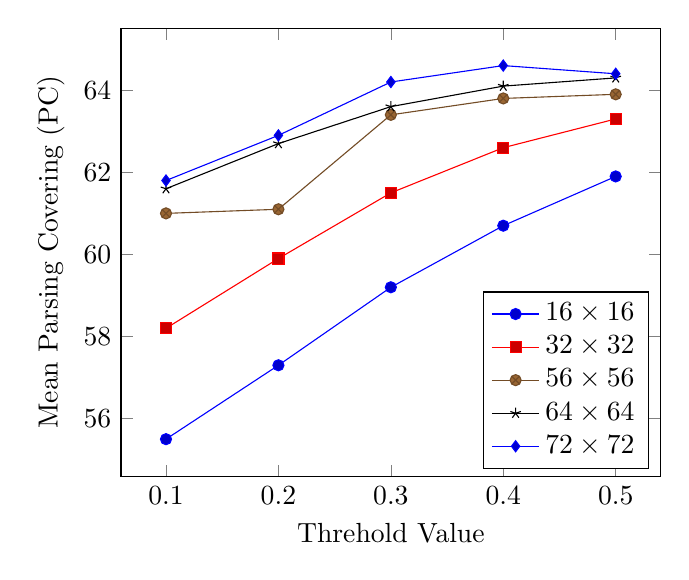
\begin{tikzpicture}
    \begin{axis}[
        xlabel=Threhold Value,
        ylabel=Mean Parsing Covering (PC),
        legend style={at={(0.67,0.215)},anchor=west}]
    \addplot plot coordinates {
        (0.1, 55.5)
        (0.2, 57.3)
        (0.3, 59.2)
        (0.4, 60.7)
        (0.5, 61.9)
    };
    \addlegendentry{$16\times16$}
    
    \addplot plot coordinates {
        (0.1, 58.2)
        (0.2, 59.9)
        (0.3, 61.5)
        (0.4, 62.6)
        (0.5, 63.3)
    };
    \addlegendentry{$32\times32$}
    
    \addplot plot coordinates {
        (0.1, 61.0)
        (0.2, 61.1)
        (0.3, 63.4)
        (0.4, 63.8)
        (0.5, 63.9)
    };
    \addlegendentry{$56\times56$}
    
    \addplot plot coordinates {
        (0.1, 61.6)
        (0.2, 62.7)
        (0.3, 63.6)
        (0.4, 64.1)
        (0.5, 64.3)
    };
    \addlegendentry{$64\times64$}
    
    \addplot plot coordinates {
        (0.1, 61.8)
        (0.2, 62.9)
        (0.3, 64.2)
        (0.4, 64.6)
        (0.5, 64.4)
    };
    \addlegendentry{$72\times72$}


    \end{axis}
\end{tikzpicture}
\label{plot:post-processingcomparison}
\caption[Post-processing Parameters Comparison ]{Comparison plot for parsing covering \gls{pc} at multiple threshold values and kernel window sizes showing a threshold value of around 0.4 and a pooling window of size $72\times72$ to be a favourable parameter choice.}}
\end{figure}

Further quantitative results corresponding to each investigated thershold level and kernel window for pooling center points has been illustrated in the table \ref{tab:parameter_comparison} below.

\sisetup{round-mode = places, round-precision = 1, scientific-notation = fixed, fixed-exponent = 0}
\begin{table}[H] % !htbp
    \centering
    \begin{tabular}{crSSSSS}
        \hline
        & & $Th_{0.1}$ & $Th_{0.2}$ & $Th_{0.3}$ & $Th_{0.4}$& $Th_{0.5}$ \\%
        \hline
        \parbox[t]{2mm}{\multirow{4}{*}{\rotatebox[origin=c]{90}{Kernel Size  }}}
        & $\mathbf{16\times16}$ & 55.5 & 57.3 & 59.2 & 60.7 & 61.9 \\
        & $\mathbf{32\times32}$ & 58.2 & 59.9 & 61.5 & 62.6 & 63.25\\
        & $\mathbf{56\times56}$ & 61.02 & 61.08 & 63.4 & 63.8 & 63.9\\
        & $\mathbf{64\times64}$ & 61.6 & 62.7 & 63.6 & 64.1 & 64.3\\
        & $\mathbf{72\times72}$ & 61.8 & 62.9 & 64.2 & \textbf{64.6} & 64.4\\
        \hline
    \end{tabular}
    \caption[Comparison of Threshold value and Pooling Kernel Window]{Table provides a comparison between various threshold values and pooling kernel window size. It can be seen that threshold of about 0.4 and pooling kernel of $72\times72$ results in best performance}
    \label{tab:parameter_comparison}
\end{table}


Comparison shows a threshold value of around 0.4 and a pooling window size of $72\times72$ to be a favourable parameter choice. Therefore, these parameters have been chosen as default for further experimentation at an early stage of evaluation.



\section{Overall Panoptic Task Evaluation}

Lessons learned from experiments with post-processing parameters have been used to select best performing settings. These parameters have been fixed for further experimentation and evaluation purposes. Therefore, a comparison after selecting these parameters has been provided in this section. Table \ref{tab:PC_overall} shows a comparison of different encoding types and center point distribution sizes with respect to class-wise parsing covering. \textit{End-End} and \textit{Center-End} represent encoding type while the number in subscript represents the distribution size used to encode the center-points.



\begin{table}[!htp] % 
  \resizebox{1 \textwidth}{!}{
  \begin{tabular}{@{}rcccccccccccccccccccc@{}}

  & \multicolumn{1}{P{90}{1.6cm}}{Road} &
    \multicolumn{1}{P{90}{1.6cm}}{Sidewalk} &
    \multicolumn{1}{P{90}{1.6cm}@{}}{Building} &
    \multicolumn{1}{P{90}{1.6cm}}{Wall} &
    \multicolumn{1}{P{90}{1.6cm}}{Fence} &
    \multicolumn{1}{P{90}{1.6cm}@{}}{Pole} &
    \multicolumn{1}{P{90}{1.6cm}}{Traffic Light} &
    \multicolumn{1}{P{90}{1.6cm}}{Traffic Sign} &
    \multicolumn{1}{P{90}{1.6cm}@{}}{Vegetation} &
    \multicolumn{1}{P{90}{1.6cm}}{Terrain} &
    \multicolumn{1}{P{90}{1.6cm}}{Sky} &
    \multicolumn{1}{P{90}{1.6cm}@{}}{Person} &
    \multicolumn{1}{P{90}{1.6cm}}{Rider} &
    \multicolumn{1}{P{90}{1.6cm}}{Car} &
    \multicolumn{1}{P{90}{1.6cm}@{}}{Truck}&
    \multicolumn{1}{P{90}{1.6cm}}{Bus} &
    \multicolumn{1}{P{90}{1.6cm}@{}}{Train} &
    \multicolumn{1}{P{90}{1.6cm}}{Motorcycle} &
    \multicolumn{1}{P{90}{1.6cm}}{Bicycle} &
    \multicolumn{1}{P{90}{1.6cm}@{}}{ \textbf{Mean}}\\
      \midrule

        $\mathbf{End-End_{8}}$ 
        &97.7&83.0&90.7&52.4&57.1&51.1&56.2&67.5&91.0&61.7&93.9&44.9&42.2&63.9&68.6&64.1&59.0&53.8&46.1&\texbf{65.0} \\
        
        $\mathbf{End-End_{16}}$ &96.0&75.0&87.4&43.6&52.8&31.1&42.7&54.4&87.2&58.4&89.7&39.4&38.6&61.7&72.9&61.8&62.1&43.7&43.3&60.1 \\
        $\mathbf{Center-End_{2}}$ &97.6&82.4&90.0&50.0&55.9&42.8&56.5&63.9&90.3&63.23&93.0&39.0&41.5&55.8&69.7&46.9&29.1&39.6&36.1&60.2 \\
        $\mathbf{Center-End_{4}}$ &97.8&83.7&90.8&52.8&54.6&50.7&59.3&68.2&91.1&63.3&93.9&42.7&43.4&61.1&66.1&61.2&64.1&42.0&36.7&64.4  \\
        $\mathbf{Center-End_{8}}$ &97.7 &83.6&90.3&52.9&53.7&48.7&54.3&66.2&90.7&61.3&93.1&45.2&41.2&64.3&73.3&65.0&66.7&40.9&38.2&\textbf{64.6} \\
        $\mathbf{Center-End_{16}}$ &96.2&76.1&88.1&44.7&49.3&35.5&50.4&58.2&89.1&60.18&91.6&43.8&37.5&59.9&63.5&52.6&30.1&37.8&36.0&57.9 \\

  \bottomrule
  \end{tabular}
  }
\caption[Overall Panoptic Task Comparison]{Comparison of different encoding types and center point distribution sizes with respect to class-wise parsing covering. Names \textit{End-End} and \textit{Center-End} represent encoding type while the number in subscript represents the distribution size used to encode the center-points.}
  \label{tab:PC_overall}
\end{table}

Comparison result suggest an appropriate size for encodings of different sizes. In general, it can be seen that smaller instances such as \textit{rider}, \textit{motorcycle} show a better performance when encoded with a smaller distribution sizes. However instances that are larger in size such as \textit{car}, \textit{truck}, \textit{bus} and \textit{train} favour a larger distribution size to encode center points. An overall best performance has been shown by encoding all the instances with a center point encoded using a guassian of standard deviation $\sigma$ = 8 pixels. 

\paragraph{Comparison with the State-of-the-Art}

Table \ref{tab:sotacomparison} shows a comparison between proposed models with xception-65 as backbone feature extractor trained on input size of $1025 \times 1025$ and batch-size = 1 with state of the art DeeperLab \cite{DBLPDeeperLab:journals/corr/abs-1902-05093}. Reported metric is \gls{pc} which is a newly proposed metric for quantifying panpotic segmentation therefore not alot of approaches have yet reported parsing covering for the evaluation of their approaches. It can be seen that proposed models with center-to-end and end-to-end encoding show a comparable performance even with smaller train crop size, partial cold start of training and a train batch size of 1 due to limited computational resources. Note that model from deeperlab uses full image resolution and manifold batch size.  
 
\begin{table}[H]
    \centering
        \begin{tabular}{cc|c} 
        \hline
            Method & Input Size  & PC $(\%)$ \\
            \hline DeeperLab - MNV2 & $513 \times 1025$  &64.66 \\
            DeeperLab - MNV2 & $1025 \times 2049$ &69.70 \\
            DeeperLab - Xception-71 &$1025 \times 2049$ &75.63 \\
            \hline (Ours) Xception-65_{c2e} &$1025 \times 1025$ &\texbf{64.6} \\
            (Ours) Xception-65_{e2e} & $1025 \times 1025$ &\texbf{65.0} \\
            \hline
        \end{tabular}
    \caption[Comparison with State of the art]{Comparison with state of the art DeeperLab with presented models at different input training sizes.}
    \label{tab:sotacomparison}
\end{table}



\section{Limitation}

Generating instance masks from center-points and offset vector representation has been employed as a simple regression problem, see section \ref{subsec:regression_approach}. Before such a grouping operation can initiate, a simple max-pooling based non-maxima suppression has been employed to get exact center locations, for more details, reader is referred to \ref{subsec:center_rendering}. It is sometimes observed that more than one mask covers a single instance. 
This behaviour has been shown in the figure \ref{fig:failurecaseexamples}

Reason for such behaviour can be explained by following reason:

\begin{enumerate}
    \item Centers predicted by the network are so dispersed that they occur in two consecutive pooling strides
    \item Center predictions occurred at the intersection of consecutive pooling filter strides.
\end{enumerate}

Illustrations of such behaviour has been visualised in the figure \ref{fig:faliurecasereason}.

\begin{figure}[H] %!htp
%\centering
    \subfigure[Failure Case 1]{
        \includegraphics[width = \textwidth / 2 ]{Graphics/Evaluations/failurecase1.png}
        \label{fig:failurecase1}}
    %\hspace{1pt}
     %add desired spacing between images, e. g. ~, \quad, \qquad, \hfill etc.
     %(or a blank line to force the subfigure onto a new line)
    \subfigure[Failure Case 2]{
        \includegraphics[width = \textwidth / 2 ]{Graphics/Evaluations/failurecase2.png}
        \label{fig:failurecase2}}
    \caption[Dual Center Pooling Illustration] {Illustration of center pooling limitation a) depicts an image showing two masks covering single instance on the left on image b) shows a small instance covered by two masks representing two center points pooled from same distribution }
    \label{fig:failurecaseexamples}
\end{figure}



\begin{figure}[H] %!htp
    \includegraphics[width = \textwidth]{Graphics/Evaluations/failurecase_reason}
    \caption[Dual Pooling of Distributions]{Illustration of two centers being pooled from one predicted distribution. Figure showing dispersed predicted distribution being pooled twice in consecutive pooling strides on the left and predicted distribution occurring at intersection of two consecutive pooling kernel strides.}
    \label{fig:faliurecasereason}
\end{figure}
\newpage
\section{Inference Times}


This section provides comparison between different backbone feature extractors against their inference times. 

Since, the feature extractor used for implementation of presented bottom-up panoptic segmentation network architecture relies on feature extractor from state of the art semantic segmentation architecture, it therefore has the possibility to use multiple backbones. Presented network architecture therefore can make use of multiple backbones depending on requirement for accuracy vs speed. It is also possible to manually reduce the maximum number of instances for segmentation by only picking the top-50 or top-200 highest predicted center-points. Therefore, table shows the inference times for both variants. 

\begin{table}[!htp]
\begin{center}

\centering



\begin{tabular}{c|c|c} 
\hline
    Backbone & Upto 200 Instances (msec)&  Upto 50 Instances (msec) \\
    \hline Xception 71 & $389$ & $281$ \\
     Xception 65 & $386$ & $263$ \\
    Xception 41 & $310$ & $191$ \\
    MobileNetv3 Large & $281$ & $162$ \\
    MobileNetv3 Small & $194$ & $102$ \\
    \hline
\end{tabular}
\end{center}
\caption[Comparison of Inference Time with Backbones]{Comparison of inference times in milliseconds incurred by different backbones for 50 and 200 instances.}
\end{table}

Reported inference times for different backbones have been recorded uisng NVIDIA RTX 2080Ti GPU.




